\documentclass[12pt]{article}

\usepackage[utf8]{inputenc}
\usepackage[T2A]{fontenc}
\usepackage[english,russian]{babel}
\usepackage{amssymb}
\usepackage{graphicx}
\usepackage{float}
\graphicspath{ {images/} }

\textwidth=431pt
\textheight=600pt
\hoffset=-30pt
\voffset=-30pt

\usepackage{graphicx}
\usepackage{amsmath}
\makeatletter
\renewcommand{\@oddhead}{%
	\vbox{%
		\hbox to \textwidth{\strut \textit{Think Math, Problem set 2, Usvyatsov Mikhail} \hfill }
		%\hbox to\textwidth{Лист\hfill Страница~\arabic{page}~из 2}
		\hrule
		\vspace{12pt}
	}}
	\renewcommand{\@oddfoot}{}
	\makeatother
	
	
\begin{document}
	\begin{center}
		\textbf{Problem set 1 \\
			DUE: Tue. September 8, 2015 \\}
	\end{center}
		
	\bigskip
	
	\textbf{Problem 1}
		In general case no, because summation of two polynomials can give us another denominator.
		In case if fixed denominator it is obviously a linear space. Its dimension is n and the basis is $\left(\dfrac{1}{q(x)}, \dfrac{x}{q(x)}, ..., \dfrac{x^n}{q(x)} \right)$. 

	\textbf{Problem 2}
		\begin{enumerate}
			\item $v_4 + v_1= v_1 + v_2 - (v_2 + v_3) + (v_3 + v_4)$, that means, that we can represent the last vector in terms of other. Thus this combination is not linearly independent. 
			\item $(v_1 - v_2) + (v_2 - v_3) + (v_3 - v_4) = -1 \cdot (v_4 - v_1)$ Thus this combination is not linearly independent.
			\item This combination is linearly independent because I cannot represent the last vector in terms of others.
			\item $ - (v_1 + v_2) + (v_2 + v_3) = (v_3 - v_4) + (v_4 - v_1)$ Thus this combination is not linearly independent.
		\end{enumerate}

	\textbf{Problem 3}
	
	According to the fundamental theorem of algebra, we can represent such polynomials in the following form: 
	$p(x) = (x - x_{-1})(x - x_0)(x - x_1) \cdot (x - x_2) \cdot ... \cdot (x - x_{n - 1})$.
	
	It means, that all vectors in this vector space will include first three guys of p(x). It means, that everything left is polynomial with degree not exceeding n - 1. Thus the dimension is n. The basis is $((x - x_{-1})(x - x_0)(x - x_1), x \cdot (x - x_{-1})(x - x_0)(x - x_1), ..., x^{n-1} \cdot (x - x_{-1})(x - x_0)(x - x_1))$
	
	\textbf{Problem 4}
	
	$A_I^1 =  \left(
		\begin{tabular}{c c}
			1 & 1\\
			1 & $-\dfrac{1}{2}$
		\end{tabular}
	\right)$
	
	$A_1^{II} =  \left(
		\begin{tabular}{c c}
			1 & 2\\
			2 & -1
		\end{tabular}
	\right)$
	
	$A_I^{II} = A_I^1  \cdot A_1^{II} = \left(
		\begin{tabular}{c c}
			3 & 1\\
			0 & 2.5
		\end{tabular}
	\right)$
		
    \textbf{Problem 5}

	For some particular B there are several possible variants: if coordinates of B are not equal there are no solutions (example (1, -1)). Otherwise there are infinite number of solutions (example (1,1)). 
	
	$\left(
		\begin{tabular}{c c}
			1 & 2\\
			1 & 2
		\end{tabular}
	\right) \cdot \left( x_1, x_2 \right)^T = (x_1 + x_2, x_1 + x_2)^T$
	
	Thus, ker(A) = $(0, 0)^T$

    \textbf{Problem 6}
    
    Yes, these matrices form a vector space. The basis is set of matrices of size (n $\times$ m) with one on $A_{ii}$ place.
    This space has dimension min(n, m) because there are min(n, m) linearly independent rows.
    
    Coordinates  of this space have the following form. 
    
    $\left( \begin{tabular}{c}
       	1\\
       	0\\
       	...\\
       	0
    \end{tabular} \right)_{min(m, n)}$.
    
    Given matrices are obviously linear independent. Yes, they form a basis over matrices two by two.
    
    $A = \left(
    \begin{tabular}{c c c c}
    $\dfrac{1}{a}$ & 0 & 0 & $\dfrac{1}{d}$ \\
    0 & $\dfrac{1}{b}$ &  $\dfrac{1}{c}$ & 0 \\
    0 & $\dfrac{1}{b}$ &  -$\dfrac{1}{c}$ & 0 \\
    $\dfrac{1}{a}$ & 0 & 0 & - $\dfrac{1}{d}$ 
    \end{tabular}
    \right)$
    
    \textbf{Problem 7}
    
    Blue whale brought me on his tale the following scalar product  <C, D> = Tr($D^TC$). Occasionally it is well defined and according to this scalar product given basis is orthonormal. For the parametrized case we can introduce <C, D> = $A^{-1}Tr((AD)^TAC$). 
    
    \textbf{Problem 8}
    
    $a_0 = \int^1_0 x - x^2 dx = \dfrac{1}{6}$\\
    $b_n = 2 \int^1_0 (x - x^2) sin(2 \pi n x)dx = 0$\\
    $a_n = 2 \int^1_0 (x - x^2) cos(2 \pi n x)dx = \dfrac{-1}{(\pi n) ^2}$
    
    \begin{figure}[H]
    	\centering
    	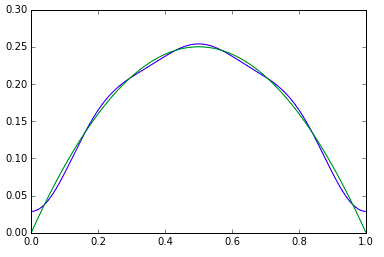
\includegraphics[width=15cm]{1}
    	\caption{"Fourier approximation"}
    \end{figure}
    
    \begin{figure}[H]
    	\centering
    	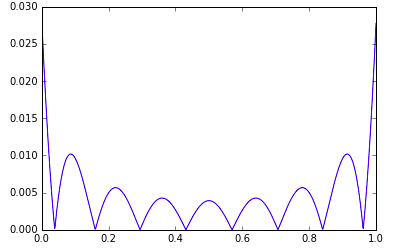
\includegraphics[width=15cm]{2}
    	\caption{"Deviation"}
    \end{figure}
    
    \textbf{Problem 9}
    
    $a_0 = \int^1_0 x dx = \dfrac{1}{2}$\\
    $a_n = 2 \int^1_0 x cos(2 \pi n x)dx = 0$\\
    $b_n = 2 \int^1_0 x sin(2 \pi n x)dx = \dfrac{-cos(2\pi n)}{n \pi}$
    
      \begin{figure}[H]
      	\centering
      	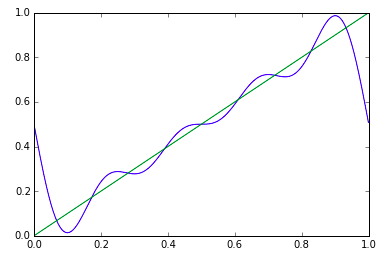
\includegraphics[width=15cm]{3}
      	\caption{"Fourier approximation"}
      \end{figure}
      
      \begin{figure}[H]
      	\centering
      	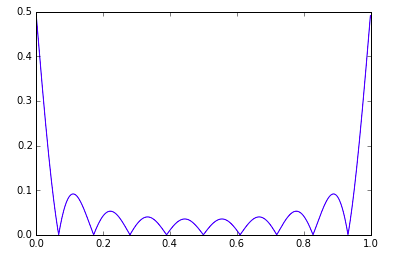
\includegraphics[width=15cm]{4}
      	\caption{"Deviation"}
      \end{figure}
    
    \textbf{Problem 10}
    
    (a b) A (a $b)^T$ = $a^2 + b^2 + 2 \lambda ab$
    Thus only if $\lambda$ = 0 there are no such a and b that can make A not positive definite.
    Eigenvector of A with $\lambda = 0$ is (a, $b)^T$ for any real a and b. 
    
    \textbf{Problem 11}
    
    Finding the characteristic polynomial gives us: $\lambda^3 - 9 \lambda^2 - 6\lambda = 0$\\
    Thus $\lambda_1 = 0$, $\lambda_{2,3} = \dfrac{9 \pm \sqrt{105}}{2}$\\
    For $\lambda = 0$ eigenvector is (1 -2 1$)^T$\\
    For $\lambda = \dfrac{9 + \sqrt{105}}{2}$ eigenvector is $(\dfrac{\sqrt{105} - 5}{10}$ $\dfrac{\sqrt{105} + 5}{20}$ $1)^T$\\
    For $\lambda = \dfrac{9 - \sqrt{105}}{2}$ eigenvector is $(\dfrac{-\sqrt{105} - 5}{10}$ $\dfrac{-\sqrt{105} + 5}{20}$ $1)^T$\\
        
    Thus  $A = \left(
	    \begin{tabular}{c c c}
		    1 & $\dfrac{\sqrt{105} - 5}{10}$ & $\dfrac{-\sqrt{105} - 5}{10}$ \\
		    -2 &$\dfrac{\sqrt{105} + 5}{20}$ & $\dfrac{-\sqrt{105} + 5}{20}$ \\
		    1 & 1 & 1
	    \end{tabular}
    \right)$.
    
    Now we can represent initial matrix as A D $A^{-1}$. Where D is diag$\left( 0 \right.$ $\dfrac{9 + \sqrt{5}} {2}$ $\left. \dfrac{9 - \sqrt{5}} {2} \right)$ 
    
    Given matrix cannot be a scalar product because it is not commutative for multiplication.
    
    \textbf{Problem 12}
    For $M_1$:\\
    $M = \left(
	    \begin{tabular}{c c}
		    1 &  0\\
		    0 & -1
	    \end{tabular}
    \right)$.
    
     $A = \left(
	     \begin{tabular}{c c}
		     1 & 1\\
		     1 & -1
	     \end{tabular}
     \right)$.
     
     For $M_2$:\\

	Its eigenvectors are zero and so it is impossible to diagonalize it.
\end{document}